\section{Propulsion Motor}
The purpose of this block is to propel the vehicle forward by turning electrical energy into rotational energy. The propulsion motor is a DC-motor. 

\subsection{Analysis}
The motor under use in this project is a Maxon produced motor, article number 370355.

The DC-motor in use, is actually a 36V motor, but due to the findings of the bachelor projekt "M7BAC\_Optimering af drivlinje", it is driven at overvoltage 48V, which increases the motors efficiency. The motor in use is specified to run at 200W. 
The motor has been modified to be able to fit inside the chassis. The modifications are length reductions to the shaft.

The figure \vref{fig:DC-motor} shows the operating range of the motor in use. It shows how to control the motor and how much the current consumption is at different RPMs.

\begin{figure}[H]
	\centering
	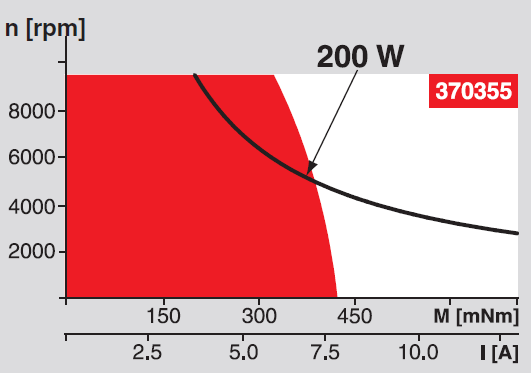
\includegraphics[width=0.6\linewidth]{Hardware/Pictures/DC-motor_diagram}
	\caption{Operating range of DC-motor in use}
	\label{fig:DC-motor}
\end{figure}

For full information concerning the motor, please refer to the datasheet. \fxnote{Husk ref}

For more information and test-resulst please refer to the documentation named "M7BAC\_Optimering af drivlinje", where there has been conducted a series of tests on the motor. 